\documentclass[10pt]{article} % Font size - 10pt, 11pt or 12pt

\usepackage[hmargin=1.25cm, vmargin=1.5cm]{geometry} % Document margins

\usepackage[usenames,dvipsnames]{xcolor} % Allows the definition of hex colors

% Fonts and tweaks for XeLaTeX
\usepackage{fontspec,xltxtra,xunicode}
\defaultfontfeatures{Mapping=tex-text}
%\setmonofont[Scale=MatchLowercase]{Andale Mono}

% Colors for links, text and headings
\usepackage{hyperref}
\definecolor{linkcolor}{HTML}{506266} % Blue-gray color for links
\definecolor{shade}{HTML}{F5DD9D} % Peach color for the contact information box
\definecolor{text1}{HTML}{2b2b2b} % Main document font color, off-black
\definecolor{headings}{HTML}{701112} % Dark red color for headings
% Other color palettes: shade=B9D7D9 and linkcolor=A40000; shade=D4D7FE and linkcolor=FF0080

\hypersetup{colorlinks,breaklinks, urlcolor=linkcolor, linkcolor=linkcolor} % Set up links and colors

\usepackage{titlesec}
\setcounter{secnumdepth}{4}

\titleformat{\paragraph}
{\normalfont\normalsize\bfseries}{\theparagraph}{1em}{}
\titlespacing*{\paragraph}
{0pt}{3.25ex plus 1ex minus .2ex}{1.5ex plus .2ex}

\usepackage{fancyhdr}
\usepackage{amssymb}
\usepackage{amsmath}
\pagestyle{fancy}
\fancyhf{}

\renewcommand{\headrulewidth}{0pt} % Get rid of the default rule in the header

\bibliographystyle{plain}

\begin{document}

\tableofcontents
\newpage

\section{Chapter: Introduction}
\subsection{What is dynein?}
\subsubsection{Basics}

Dynein is a cellular structure which converts chemical energy to mechanical energy. It does so by reacting with adenosine triphosphate (ATP) to take steps along long cellular tracks known as microtubules (MTs). Dynein's mechanical energy is used to transport molecules around the cell, pull chromosomes during division, move cellular propellers known as cilia and various other functions \cite{cianfroccoreview}.\\

Dynein is a protein with many smaller domains. A depiction of the protein and its labeled subdomains is shown in Figure (\ref{dynein-artist-rendition}). Each motor is a homodimer made up of two identical monomer proteins. Each monomer has a binding domain which binds to the microtubule, a motor domain which binds ATP, a tail domain which connects to the other monomer, a stalk which connects the binding and motor domains, and a linker which connects the motor and tail domains. The tail domain is also responsible for binding to cargo.\\

\begin{figure}[h]
  \centering
  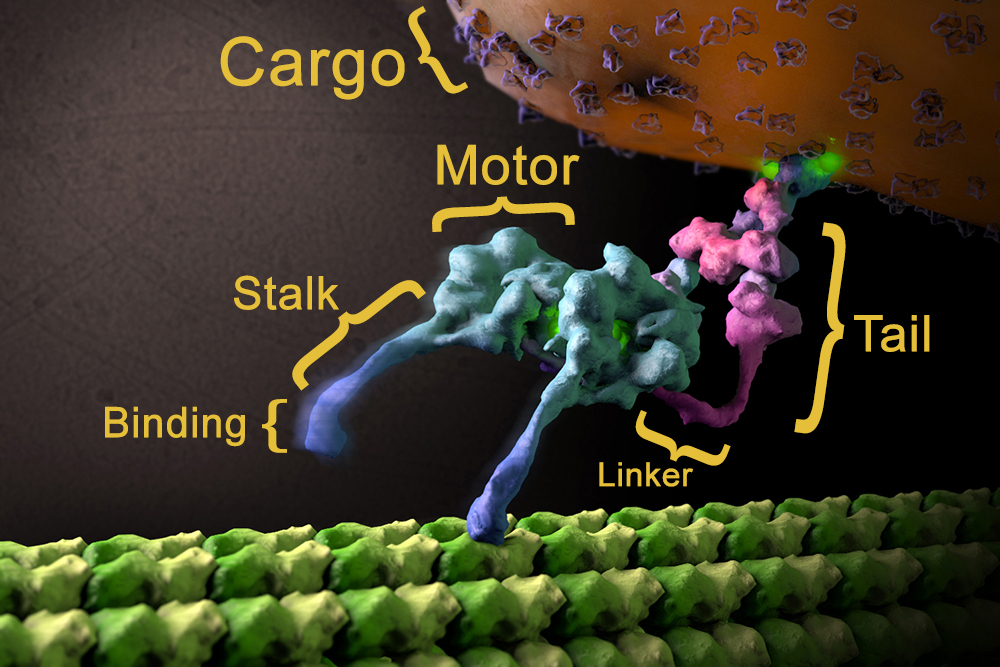
\includegraphics[width=.65\textwidth,keepaspectratio]{../figures/dynein-artist-rendition.jpg}
  \caption{Artist rendition of the dynein motor bound to a microtubule. One monomer is bound to the MT, and one is raised up. Modified. Source: Lander Lab, The Scripps Research Institute.}
  \label{dynein-artist-rendition}
\end{figure}

Dynein is believed to move by using the energy of ATP to cycle through a ring of states, each with different spatial relations to the microtubule. By cycling forward through this ring, the molecule can end up in the same state it began, but moved forward a small amount. This ring of states is known as the mechanochemical cycle \cite{cianfroccoreview}. The goal of this project is to create a mathematical model of the mechanochemical cycle and verify that it can reproduce experimental dynein stepping data. There are several types of dynein which all behave differently. This project will focus on cytoplasmic dynein-1, hereby referred to as dynein.\\

\subsubsection{Glossary}
\textbf{ATP} Adenosine triphosphate is a small organic molecule which very spontaneously breaks apart into ADP and a phosphate. This reaction is used to power many energy-requiring mechanisms within the cell. This reaction has a $\Delta G^\circ \approx -36 kJ/mol$ at physiological conditions \ref{ATPenergy}.\\\\
\textbf{Protein} Dynein is a protein, or long chain of amino acids linked together and folded into a particular shape.\\

\subsubsection{Why do cells need motor transport?}
Cells are organized, heretogenous structures which respond quickly to their environments. This means that cells require a mechanism for rapidly moving components to precise locations within the cell. This can be a challenge, since cells are fairly large compared to the proteins which compose them. A human fibroblast cell has a volume of roughly 2000 $\mu m^3$\cite{fibroblastvolume}, corresponding to roughly $8 \mu m$ in diameter. In comparison, human hemoglobin has a diameter of roughly $5 nm$ (PDB id 5ME2) \textbf{((is this the best way to cite this?))}, a $10^3$ factor difference in size.\\

Diffusion, or random motion of molecules due to collisions with solvent (i.e. Brownian motion), is one possible process cells could use to transport biomolecules. Diffusion has two problems: it is slow and nondirected. The expected distance covered for one-dimensional Brownian motion after time t was found by Einstein to be \textbf{cite here}:

\begin{equation}
  \label{diffusion-equation}
  <x> = \sqrt{2Dt}
\end{equation}

where D is the diffusion constant describing the diffusability of the biomolecule. For a medium-sized (140kD, 1D = weight of H atom) protein with a diffusion constant $D = .2 \mu m^2/s$ \cite{diffusionconstants}, it would take about a month to travel across a millimeter-sized cell. In contrast, it would take dynein, which travels at roughly 100nm/s \cite{weihongpaper}, a much more reasonable three hours to do the same.

\begin{figure}[h]
  \centering
  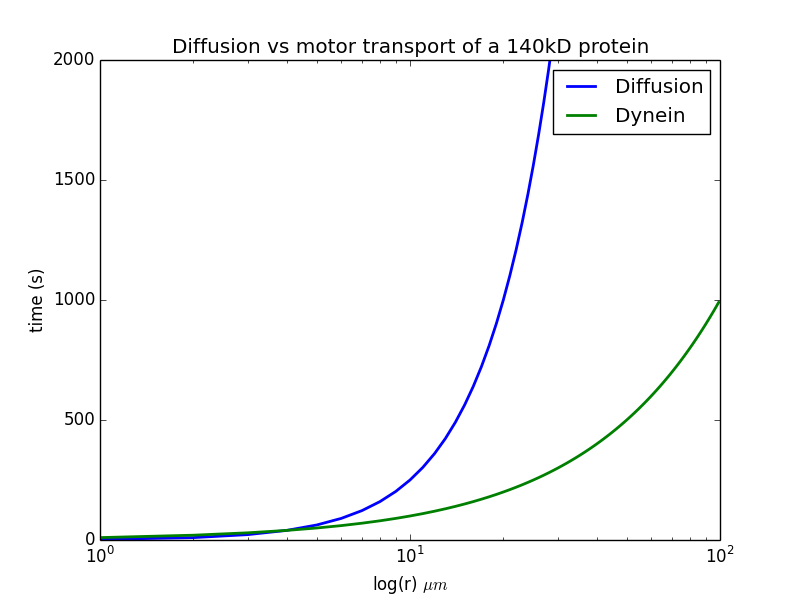
\includegraphics[width=.65\textwidth,keepaspectratio]{../figures/diffusion_vs_dynein.png}
  \caption{Plot comparing the diffusion rate of a 140kD protein with a diffusion consant $D = .2 \mu m^2/s$ with a dynein motor travelling at 100nm/s.}
  \label{diffusion_vs_dynein}
\end{figure}

\textit{Maybe use the more reasonable 2$\mu m / s$ number for dynein velocity, in-vitro speed may not be applicable since [ATP]-limited}

Another advantage of motor transport is that microtubules can be highly specific in their location in the cell. During cell division chromosomes line up at the center of each cell in a plane. Such a geometrically precise shape requires some sort of directed motion which a random process could never provide.\\

\textit{maybe decorate the above plot with pictures of cells of each size, or how long certain cellular events take? That could be cool and make it actually an interesting plot}
\textit{this argument would be much better if you could find examples of things which need to be done quickly in the cell, like responding to foreign particles or signalling
  molecules or cell division or neural events}

\subsubsection{What role does it play in the cell?}
Some of dynein's primary roles in the cell are to transport cellular cargos such as organelles, vesicles, mRNA, cytoskeletal filaments and certain proteins. Dynein also plays a role in positioning and breaking down the nucleus, cell death, spindle formation and the placement of other important cellular structures \cite{valetoolbox}.

Microtubules are long polymers of alternating $\alpha-$ and $\beta-$ tubulin subunits. MTs are polar, meaning they have a distinct directionality based on the orientation of thetubulin proteins which comprise them. One pole, the minus end, is where they initiate formation, typically at a MTOC (microtubule organizing center) around the center of the cell. The other pole, the plus end, is where they grow and shrink from. Kinesin and myosin, two other families of motor protein, typically walk towards the plus end of the MT. Dynein is unique in that it walks towards the minus end, making it a minus end-directed motor. This lends it to a particularly important function inside neurons known as retrograde transport.\\

Neurons have cell bodies at their centers and axons which grow outwards. Axons are long, narrow structures extending up to a meter in length in humans. Cell bodies contain nuclei and important organelles for synthesizing proteins, but growth of axon tips is vital for neuron function. This means bidirectional motor transport between axon tips and cell bodies is very important in neurons, since diffusion would not be quick enough. Retrograde transport is transport from the axon tip to the cell body. Cargo includes vesicles full of proteins ready to be broken down in the cell body and microtubule fragments to be returned from the axon tip \cite{neuroanatomy}. Because microtubule minus ends are found in the cell body, dynein's minus end-directed nature makes it the only protein capable of retrograde transport. An interesting question is, if proteins like dynein are synthesized in the cell body but needed at the axon tip to perform retrograde transport, how do dynein get to the tip? The answer is shown in \ref{retrograde-transport}: kinesin, a plus end-directed motor, takes dynein to the tip from the cell body.\\

\begin{figure}[h]
  \centering
  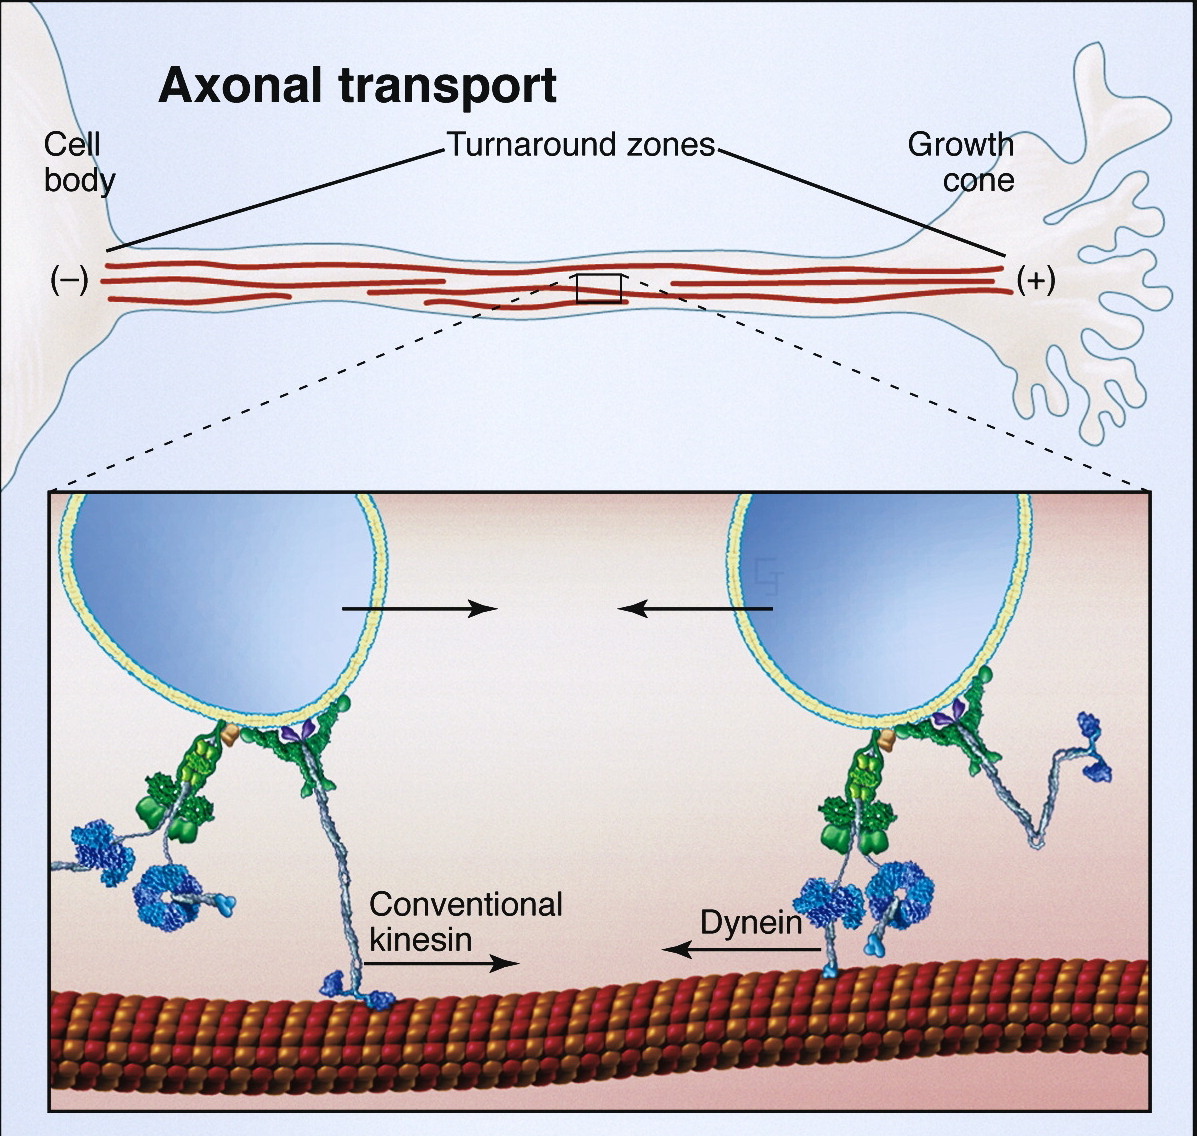
\includegraphics[width=.65\textwidth,keepaspectratio]{../figures/retrograde_transport.jpg}
  \caption{Mechanism of dynein localization to axon tips, or growth cones, in retrograde transport mediated by kinesin anterograde transport. Modified from \cite{valetoolbox}.}
  \label{retrograde-transport}
\end{figure}

\subsubsection{Dynein structure}

\begin{figure}[h]
  \centering
  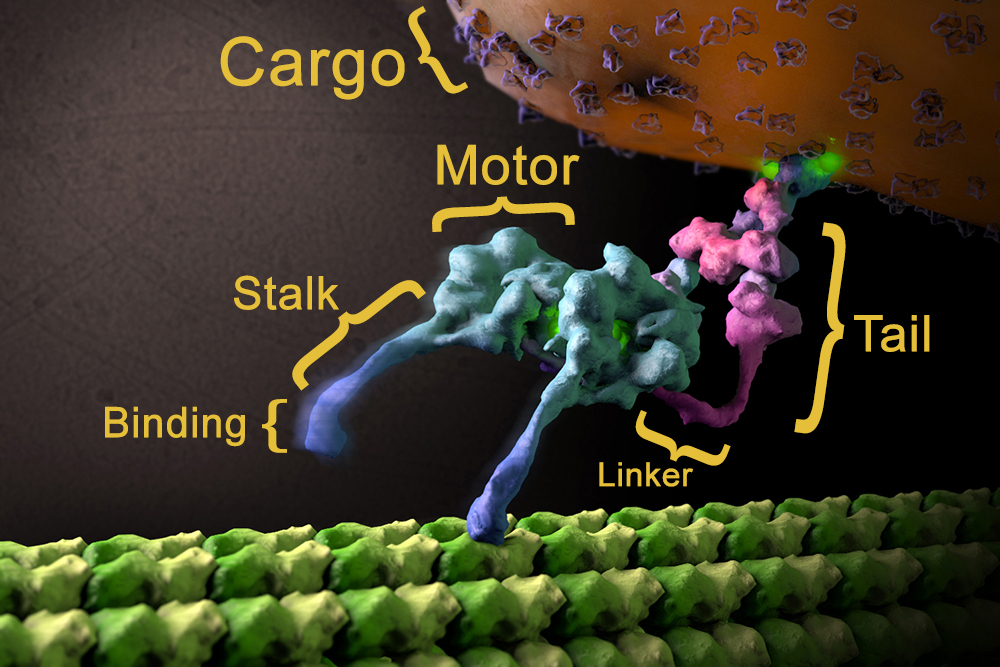
\includegraphics[width=.65\textwidth,keepaspectratio]{../figures/dynein-artist-rendition.jpg}
  \caption{Artist rendition of the dynein motor bound to a microtubule. One monomer is bound to the MT, and one is raised up. Modified. Source: Lander Lab, The Scripps Research Institute.}
  \label{dynein-artist-rendition-2}
\end{figure}

\textit{eventually find a different figure}

As shown in \ref{dynein-artist-rendition-2}, a dynein motor is a fusion of to identical subunits, or monomers, each with binding, stalk, motor and tail subdomains. Each of these subunits has a unique purpose for the motor.

\textbf{Binding domain}
Microtubule binding domains (MTBDs) allow dynein to bind to the microtubule. 

\begin{figure}[h]
  \centering
  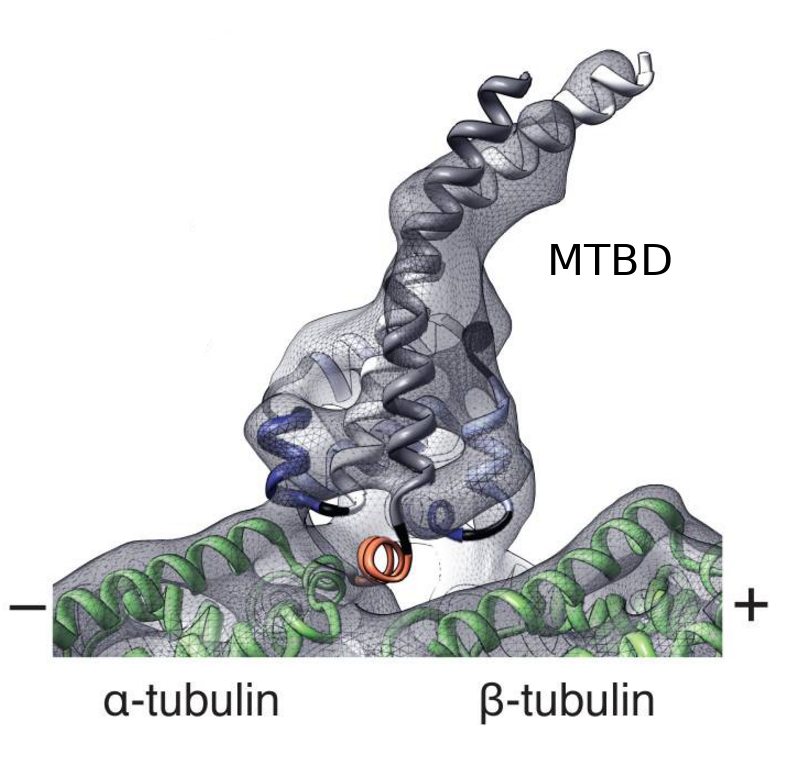
\includegraphics[width=.65\textwidth,keepaspectratio]{../figures/mtbd-complex.png}
  \caption{Crystal structure of the MTBD-MT complex. Modified from Redwine \textit{et. al} \cite{redwineMTBDcomplex}.}
  \label{dynein-artist-rendition-2}
\end{figure}

\subsubsection{How does it behave?}
Talk about its stepping behavior using Weihong's figures (as well as the new paper David found?)\\

Also possibly talk about the other things Dynein has been found to do, such as hydrolyse ATP and
move its subdomains around. This may be better in a different section than the introduction though,
since its a lot of biochemistry for the second section in an intro? maybe not, it has to go somewhere.

\subsubsection{Why is dynein special and interesting?}
Compare the processive motion of dynein to kinesin in \textbf{a.)} directionality, \textbf{b.)}
stepping pattern and \textbf{c.)} size (like how it can step over roadblocks kinesin cannot).\\

Talk about why a random stepping motor is interesting compared to a orderly-stepping motor: what
is different about dynein's structure that makes it step differently? Compare the crystal structures
and ask lots of questions. Build interest in the motors here.\\

%% \begin{figure}[h]
%%   \centering
%%   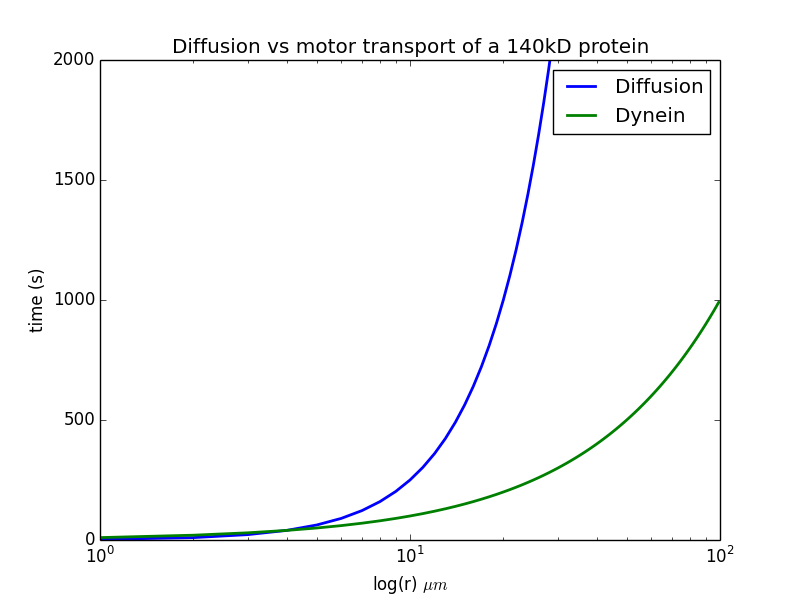
\includegraphics[width=.65\textwidth,keepaspectratio]{../figures/diffusion_vs_dynein.png}
%%   \caption{Crystal structures of cytoplasmic dynein 1 and kinesin KIF5B (PDB IDs 4RH7 and 1BG2).}
%%   \label{kin_n_dyn}
%% \end{figure}

\textit{make this figure good -- find a full length kinesin crystal structure, not 1BG2. Use kindyn.pse as a template.}

\subsection{How does dynein walk?}

Cianfrocco \textit{et. al} \cite{cianfroccoreview} propose dynein achieves motion via transitioning through the cycle of states shown in Fig. \ref{mech-cycle}. This model will hereon be referred to as the Cianfrocco model. The model claims the primary events in the dynein step are as follows. First, starting with both binding domains attached to the MT, ATP binds to the motor domain, which causes it to change conformation. This change causes the binding domain to release the microtubule, meaning only one binding domain is MT-bound. The free binding domain then undergoes another conformation change known as the ``priming stroke,'' which changes the orientation of the binding domain with respect to the MT. Finally the binding domain rebinds to the MT, causing a final conformation change in the motor which returns it to the beginning of the cycle. The exact order of these events is not precisely known. More detail on each step of the cycle is given below.\\

\textbf{Things which are known about dynein which support the Cianfrocco model}
\begin{itemize}
\item AAA1 only ATPase necessary for motility \cite{cianfroccoreview}
\item AAA5 mediates stalk register changes Schmidt H, Zalyte R, Urnavicius L, Carter AP. 2014. Structure of human cytoplasmic dynein-2 primed for
  its power stroke. Nature 518:435–38
\item Linker moves as response to AAA1 nucleotide binding Burgess SA, Walker ML, Sakakibara H, Knight PJ, Oiwa K. 2003. Dynein structure and power stroke. Nature
421:715–8
\end{itemize}

\begin{figure}[h]
  \centering
  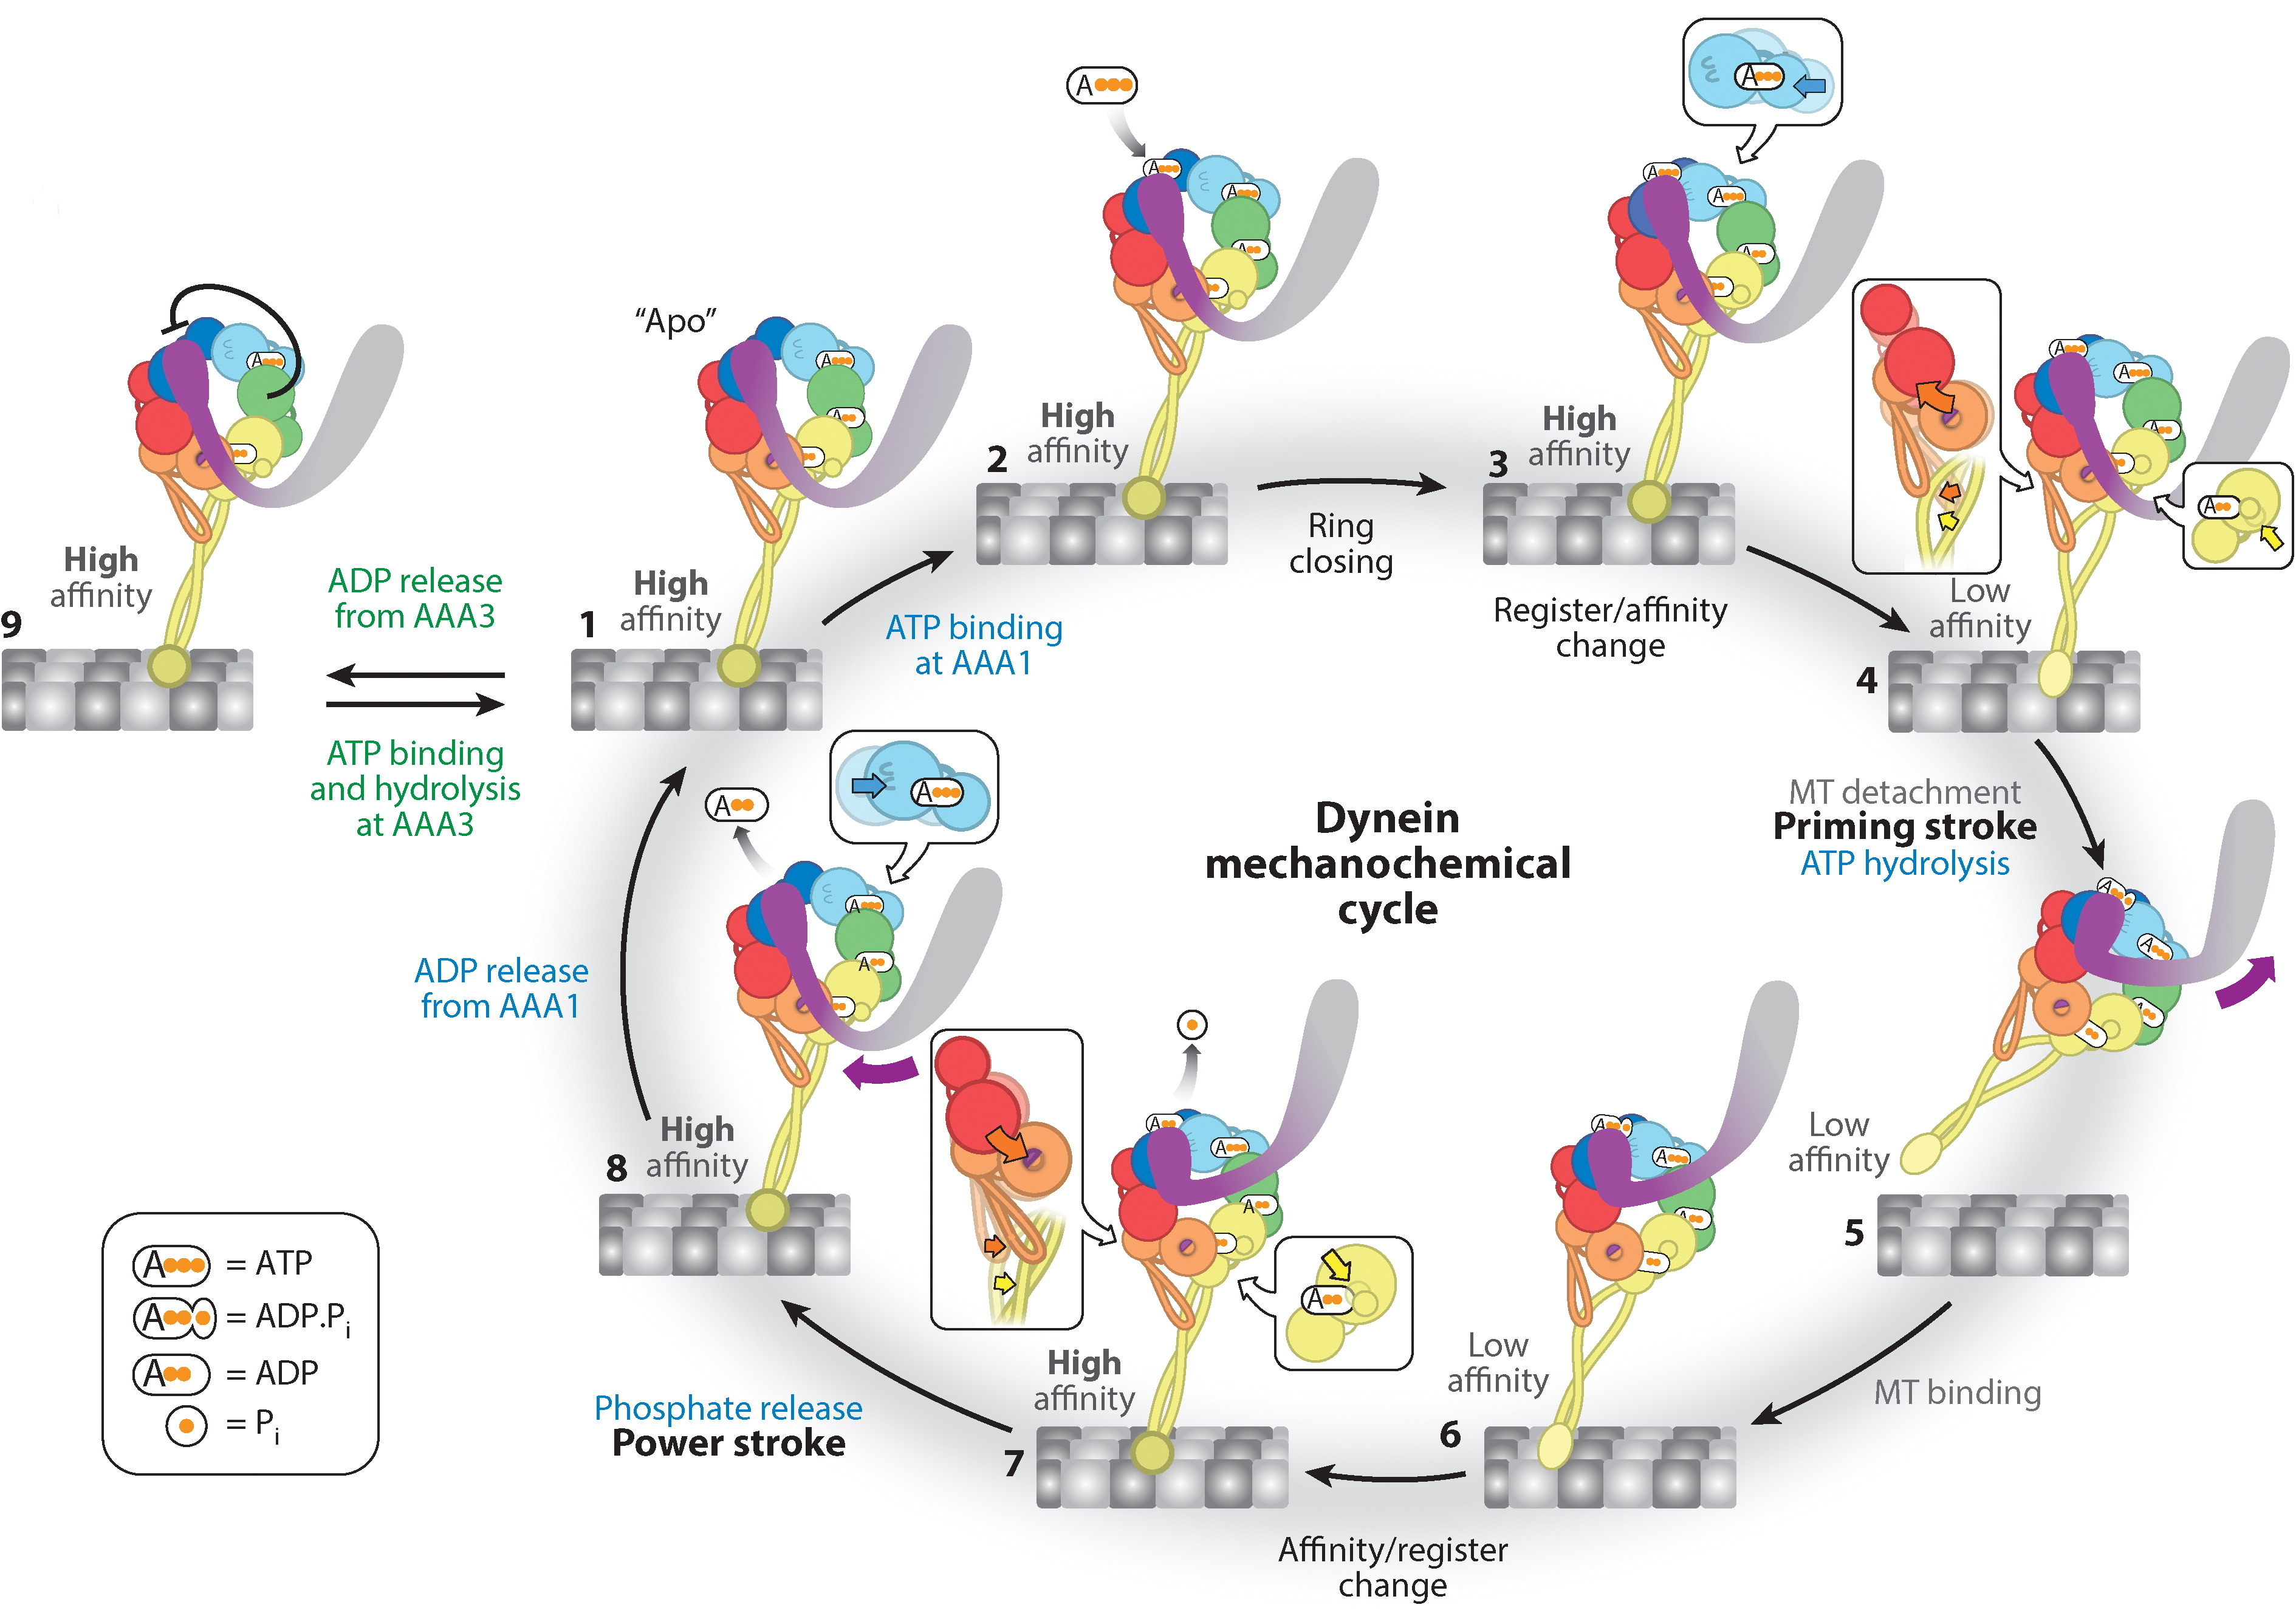
\includegraphics[width=.65\textwidth,keepaspectratio]{../figures/mechanochemical-cycle.png}
  \caption{Cycle of states the dynein motor goes through during motion in the Cianfrocco model \cite{cianfroccoreview}.}
  \label{mech-cycle}
\end{figure}

\subsubsection{ATP binding}

\subsubsection{Experimental results on dynein’s step}
Weihong's figures go here.\\
\subsubsection{Experimental features of dynein (ATPase, multi-state…)}
Some history of studies which have determined what dynein has in it.\\

\subsubsection{Powerstroke Theory}
Talk about the history of this idea, why it is supported and why it is not supported.\\
\paragraph{The theory}
Describe the theory.
\paragraph{b Evidence of theory}
Evidence supporting the powerstroke.

\subsubsection{c What is still needed to support theory}
Where our simulation fits in. Why we need this kind of information.
\subsubsection{Other theories?}
Imamula model, how it is different from Cianfrocco model, and why we chose teh Cianfrocco model.\\
	\subsection{Past Simulations}
		\subsubsection{Why simulations are necessary}
		\subsubsection{Sarlah Winch Model}
		\subsubsection{-x Other models}
	\subsection{Brownian motion}
                \subsubsection{Introduction/derivation}
                \subsubsection{Justification}

\section{Chapter: Methods}
\subsection{Simulation}
Talk about why simulation is the only way to verify the mechanochemical cycle, since experiments
aren't high resolution enough to make good videos of the walk, and even if they were, in some sense
knowing that dynein behaves identically to a simple mathematical model is more informative than
a video, since there is lots of information in a video and really precise info in a simulation.\\

\textbf{Not sure where this goes:} The 'goal' of our experiment, at a very high level, is to
understand how dynein works. We can know this if we can come up with the minimum set of characteristics a physical system needs to act like dynein. This information is the same thing as knowing
``how dynein walks.'' We don't need to know all the complex dynamics of every single amino acid in
dynein, we only need to know our rough model.\\

\subsection{Our model}
Talk about what the important parts of the mechanochemical cycle from the introduction are, and how
we take those and model them.\\
\subsubsection{Rigid point model}
Talk about two things: reducing bulky circular domains to points (is this the same as unified atom
model?) with a certain drag constant based on radius, and acting like the domains are rigid in
distance from each other. Talk about why this is valid (is it? it's an assumption, David may know
more).
\subsubsection{Harmonic energies}
How we're modeling the complicated folding and adjusting of a massive protein as a harmonic
oscillator. Why this is valid. Also other approaches...what else could we have modelled it as?
\subsubsection{Two-state model}
The mechanochemical cycle has eight states. We choose two as representative because \textbf{a.)}
many of the states are identically conformationally or \textbf{b.)} the transitions happen so fast
the intermediate states don't matter. Talk about rate constants here.
\subsubsection{Limitations}
Talk about the things we \textit{don't} take into account...motor-motor interaction, 2d information,
other ATPase nucleotide state, saying certain mechanochemical steps occur ``fast,'' not taking into
account all mechanochemical cycle states, making the coiled coil domain rigid even though it may be
springy...

\subsection{Simulating our model}
Talk generally about what simulating stuff means.\\
\subsubsection{Motion equations}

\paragraph{a Onebound solution}
Discuss how our model is represented by the following figure (maybe get one with springs on the
hinges):\\

\begin{figure}
  \centering
  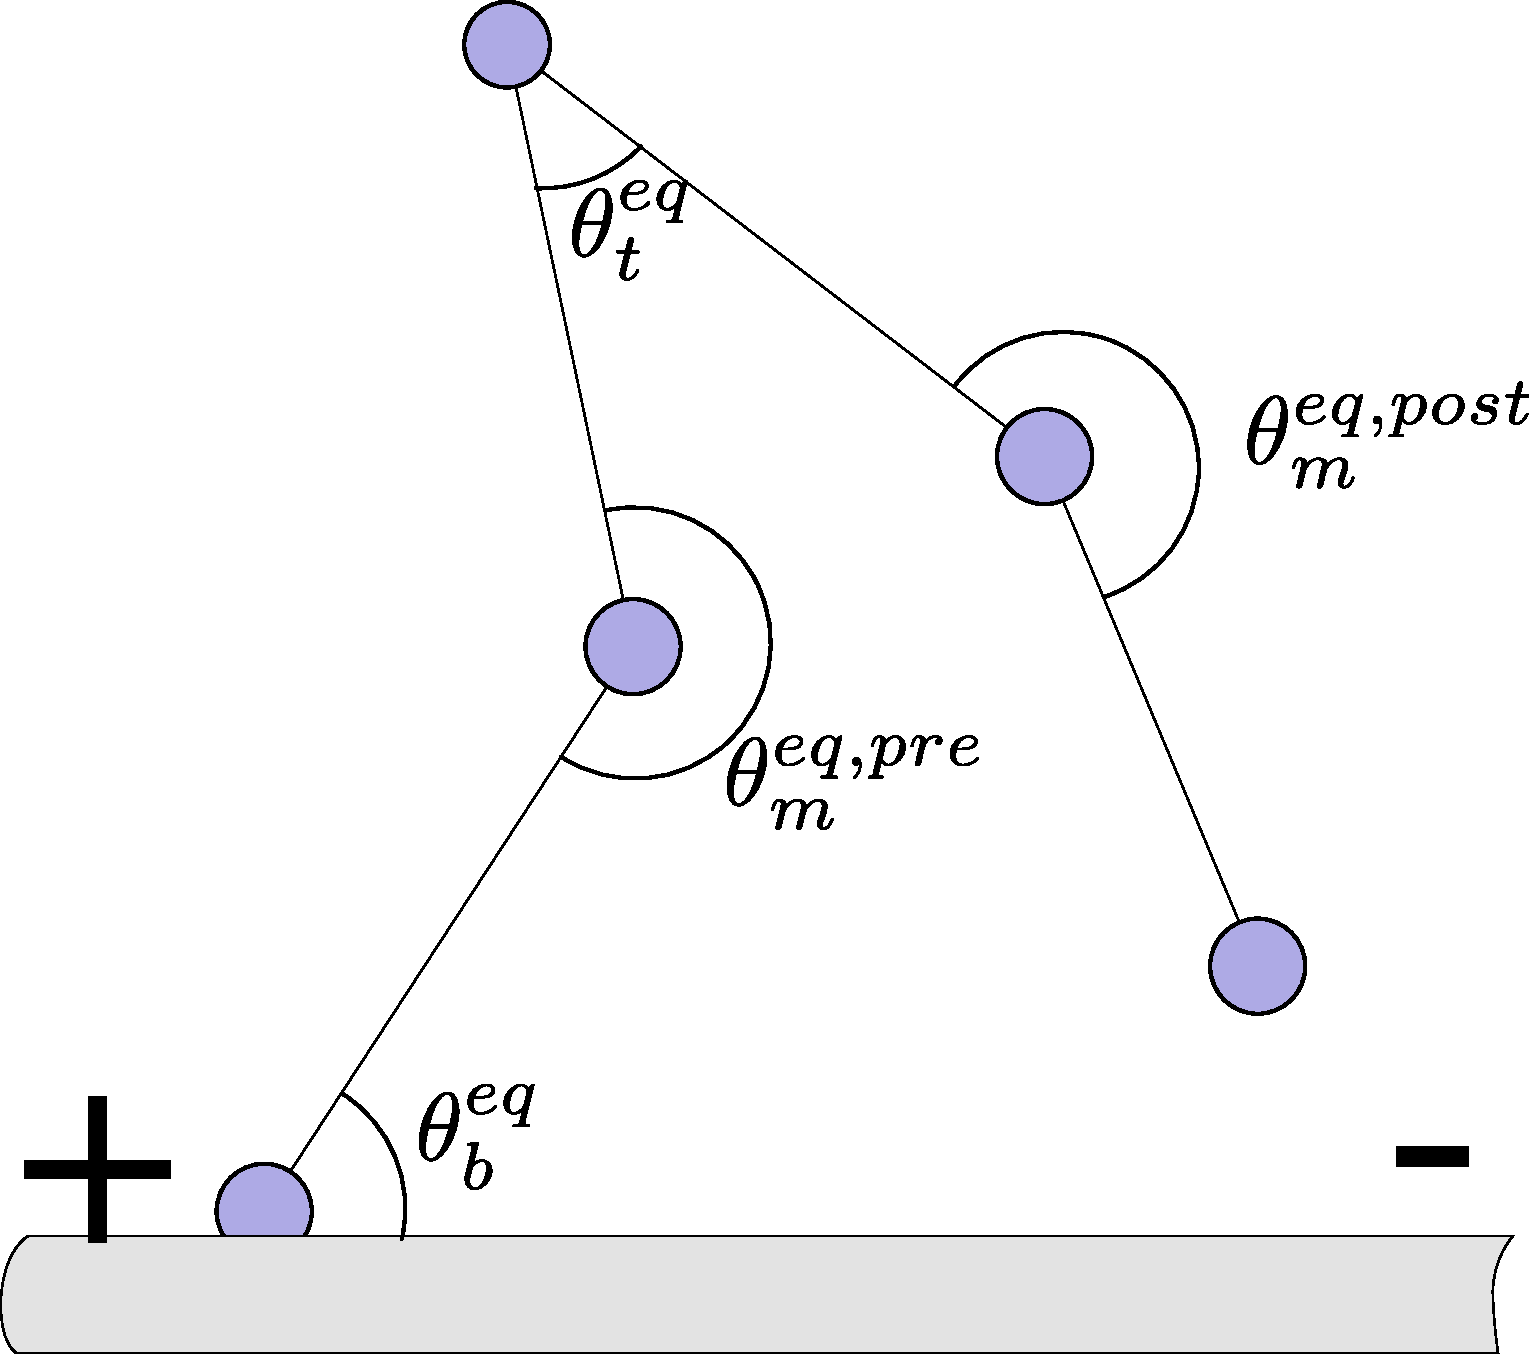
\includegraphics[width=.45\textwidth]{../figures/equilibrium-onebound}
  \caption{Definition of equilibrium angles.}
  \label{fig:eq_angles}
\end{figure}

Show the derivation process.\\

\paragraph{b Bothbound solution}
Show how bothbound is derived and different from onebound. Put the actual equations in the appendix,
or just leave them out 'cause they're ugly?\\

\subsubsection{Code}
Talk about using C++, Make, C, Python. Talk about the rough program flow, how we go from code to
data.\\

\paragraph{a Running, compiling, language choice?}
Details on why we chose C++.\\
\subsubsection{Time evolution}
How we do time evolution.
\paragraph{Euler’s method}
Show how Euler's method is arrived at, how its error scales, why we use it.

\paragraph{Vs other methods (Runge Kutta, etc)}
Talk about why our differential equation is most conducive to Euler's method. Euler's is more
efficient -- is there a way to show how our differential equation is smooth, not jagged?

\paragraph{Finding the right dt}
Figure on error rate vs. dt.

\paragraph{State transitions}
Talk about how we calculate transition rates based on differences in energies between states.
Then how we use transition rates to transition our model accurately.\\

\paragraph{Gibbs energy of transition}
Do some stuff with Gibb's here? Why our energies are Gibb's and not internal energy?\\

\subsection{Verifying our model}
Talk about why we think our model accurately represents the system we are trying to model, and
doesn't have bugs in it.\\

Talk about this figure:

\begin{figure}[h!]
  \centering
  \begin{minipage}[b]{0.49\textwidth}
    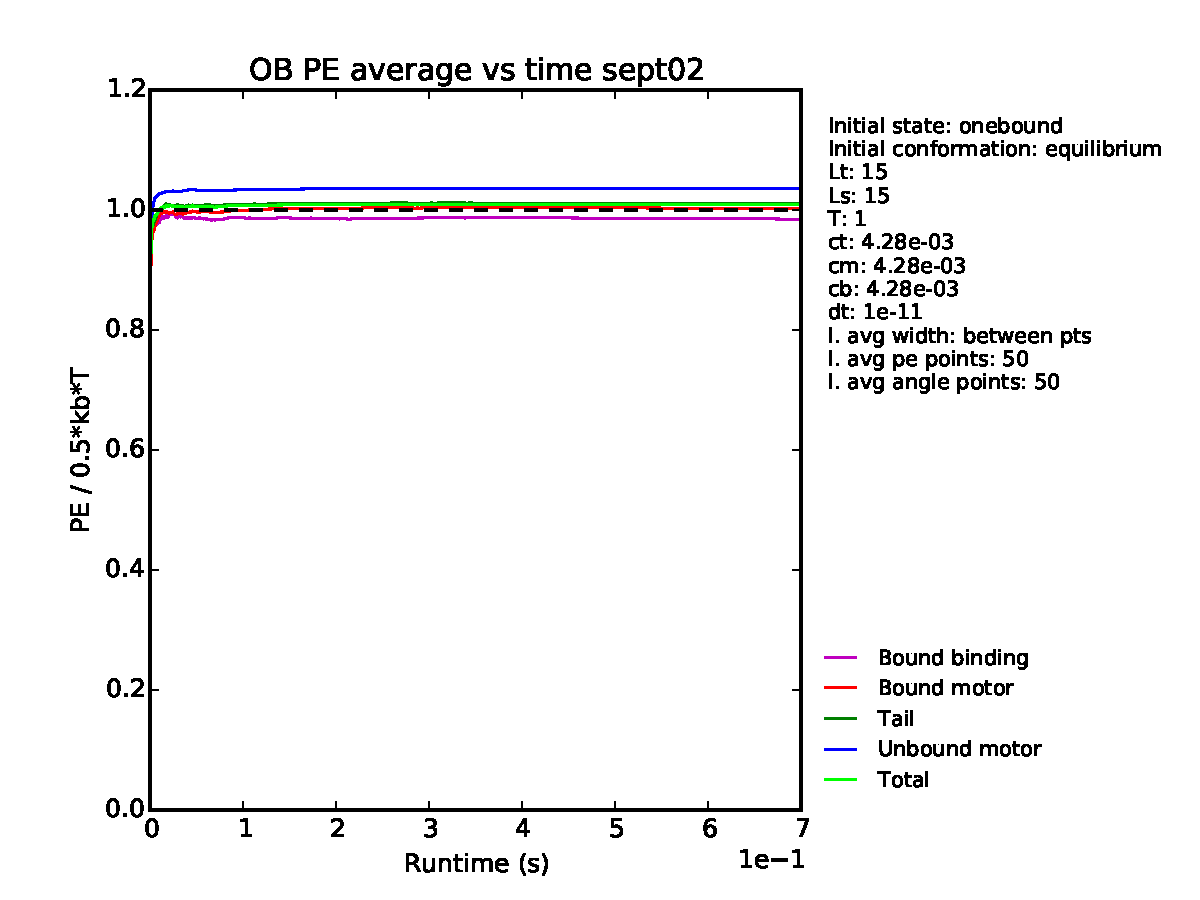
\includegraphics[width=\textwidth]{../figures/OB_Average_PE.pdf}
    \caption{Onebound PE vs time.}
  \end{minipage}
  \begin{minipage}[b]{0.49\textwidth}
    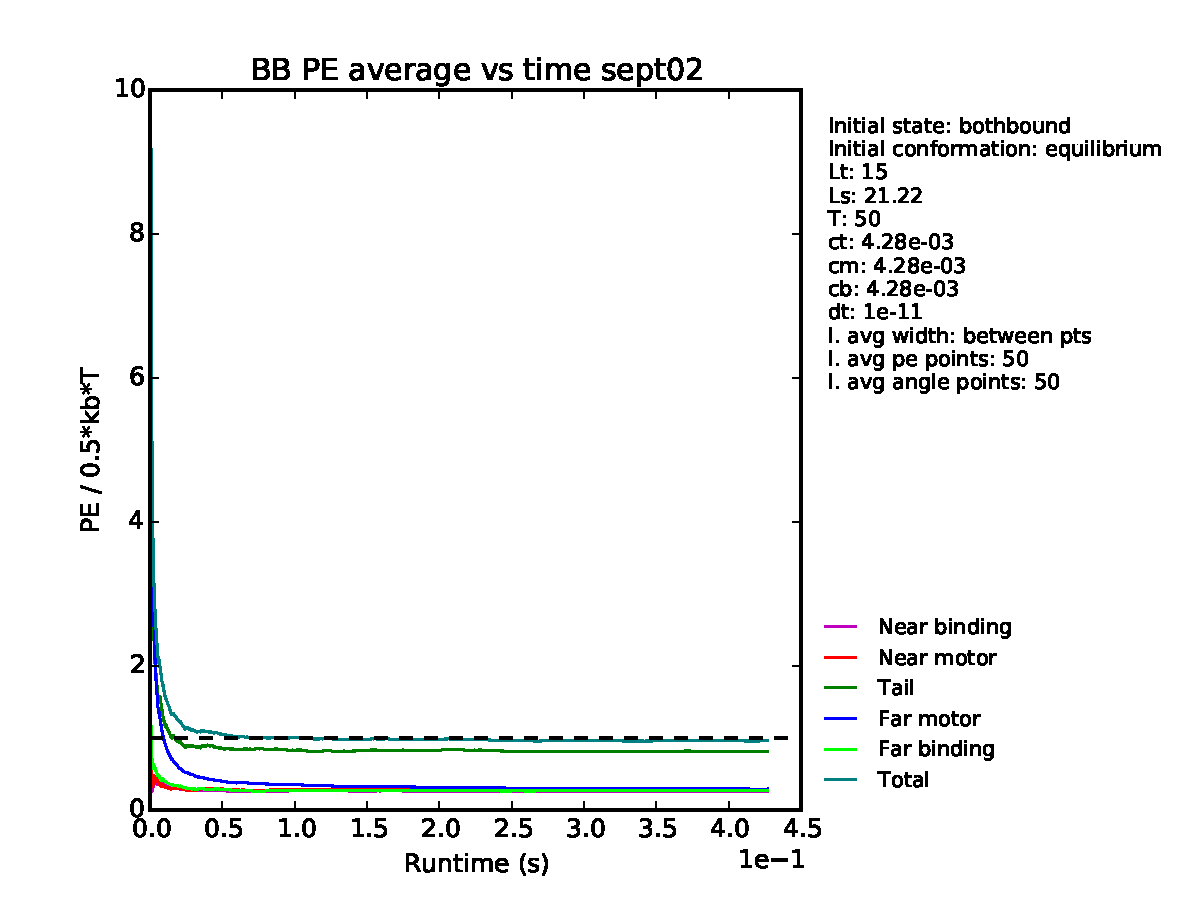
\includegraphics[width=\textwidth]{../figures/BB_Average_PE.pdf}
    \caption{Bothbound PE vs time.}
  \end{minipage}
  \label{fig:equipartition_agreement}
\end{figure}

and how it shows our model is physical, or at least, how obeying the equipartition theorem shows
how our domains both feel harmonic energies and can fully explore their spaces?\\

\subsection{Parameters}
The following table shows our guess parameters from various papers/crystal structures.\\
                        
                        \begin{center}
  \begin{tabular}{| l | l | l | l | l | l |}
    \hline
    & Winch (Sarlah) & Schmidt & Lin & PyMol 3VKH & PyMol 4RH7\\\hline
    $L_s$ & 12nm & & & 21.0nm & 22.1nm\\ \hline
    $L_t$ &  7nm & & & & 11.15nm\\ \hline
    $R_b$ &  & & & 1.57nm & 1.45nm\\ \hline
    $R_m$ &  7nm & & & 7.36nm & 6.3nm\\ \hline
    $R_t$ &  & & & & 2.16nm \\ \hline
    $\theta_{m}^{Pre}$ & 250$^{\circ}$ & & 171$^{\circ}$ & &\\ \hline
    $\theta_{m}^{Post}$ & 330$^{\circ}$ & & 137.5$^{\circ}$ & &\\ \hline
    $\theta_{b}$ & 56$^{\circ}$ & & 63.5$^{\circ}$ & &\\ \hline
    $\theta_{t}$ & 0$^{\circ}$ & & & &\\ \hline
    $k_{ub}$ & $180 s^{-1,a}$ & & & &\\ \hline
    $k_b$ & $5000 s^{-1,b}$ & & & &\\ \hline
  \end{tabular}
\end{center}
		\subsubsection{Lengths, angles, binding constants, etc…}
	\subsection{Tuning our model}
	\subsubsection{Searching for optimal parameters}
\section{Chapter: Results}
	\subsection{Histograms}
		\subsubsection{Step length histograms}
		\subsubsection{Step time histograms}
	\subsection{Other ways to represent data?}

\section{Chapter: Discussion}
\subsection{Why our model worked, didn’t work}
Fill this out over winter when you know more.\\
\subsection{Future work on this project}
If setbacks happen, this'll be a big section. Or, further simulations which could be done.

\subsubsection{Experiments to verify our model}
Talk about how FRET could be used to verify our model. We have domain distance info over long
timescales in our model - this is something we could compare to a FRET experiment exploring
the distance between domains in dynein.\\

Other biophysics experiments which could verify our model?\\

Calorimetry could get Gibb's energy of binding if you froze the motor in onebound using
vanadium? Maybe...\\
\subsection{Possible further projects}
\subsection{Difference between dynein and kinesin}
Our project un/successfully predicted how dynein behaved. How would we modify it to describe kinesin?
Is dynein's linker-motor connection less tense than kinesin's, leading to more random motion? This
would likely be lots of speculation, but it could be cool to look up some papers on kinesin motility
and get its crystal structure to do some comparisons.

\bibliography{thesis-articles}

\bibliography{thesis-webpages}

\section{Questions for Tate/Nicole}
\begin{itemize}
\item How responsible am I for the papers I cite? Should I have read them, know their methodologies?
\item Is it appropriate to cite web pages in a thesis? In a separate citation section?
\item When is a fact ``common knowledge'' enough that it doesn't need a citation?
\item Some papers have 'Request permission to reuse' links - do I need to do this for copying figures?
\end{itemize}
\end{document}
